\subsubsection{UCS 6 - Selezione del monitoraggio di un'organizzazione o di un luogo specifico}%kite level

\begin{figure}[h]
\centering
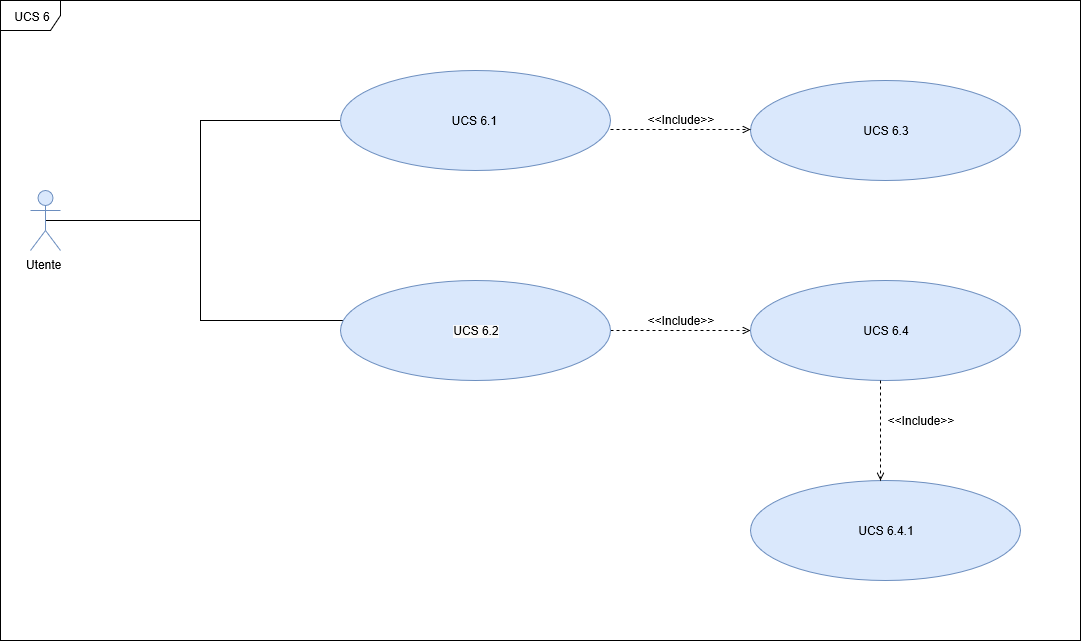
\includegraphics[scale=0.3]{sezioni/UseCase/Immagini/UCS6.png}
\caption{Selezione del monitoraggio di un'organizzazione o di un luogo specifico}
\end{figure}

\begin{itemize}
\item \textbf{Attori primari:} Amministratore visualizzatore;
\item \textbf{Precondizione:} L'amministratore deve essere autenticato presso il sistema;
\item \textbf{Postcondizione:} L'amministratore avrà visualizzato il numero di utenti anonimi presenti in un'organizzazione o in un luogo specifico;
\item \textbf{Scenario principale:} L'amministratore, dopo aver selezionato l'organizzazione, accede alla funzionalità di monitoraggio di un'organizzazione o di un luogo specifico per poter visualizzare il numero di utenti anonimi presenti al suo interno;
\item \textbf{Flusso di eventi:}
\begin{enumerate}
	\item UCS 3 - L'amministratore ha selezionato l'organizzazione; ???
	\item L'amministrazione deve selezionare la funzionalità di monitoraggio del luogo;
	\item L'amministratore può selezionare la funzionalità di un luogo specifico (6.4.1);
	\item L'amministratore deve selezionare la funzionalità di conferma (UCS 6.3);
	\item L'amministratore può visualizzare gli utenti anonimi di un'organizzazione (UCS 6.1) o può visualizzare gli utenti anonimi di un luogo specifico (UCS 6.2);
\end{enumerate}
\item \textbf{Estensioni:}  Visualizzazione di un messaggio che informa l’indisponibilità del server [?????];
\item \textbf{Inclusioni:}
\begin{enumerate}
	\item UCS 3 l'amministratore ha selezionato l'organizzazione;
\end{enumerate}
\end{itemize}

\subsubsection{UCS 6.1 - Visualizzazione del numero di utenti anonimi di un'organizzazione}%sea level
\begin{itemize}
\item \textbf{Attori primari:} Amministratore visualizzatore;
\item \textbf{Precondizione:} L'amministratore si trova nella sezione di monitoraggio;
\item \textbf{Postcondizione:} L'amministratore ha visualizzato il numero di utenti anonimi contenute nell'organizzazione scelta;
\item \textbf{Scenario principale:} L'amministratore deve aver scelto la funzionalità di conferma per poter visualizzare il numero di utenti anonimi presenti nell'organizzazione scelta;
\item \textbf{Flusso di eventi:} 
\begin{enumerate}
	\item UCS 6.3 L'amministratore deve aver scelto la funzionalità di conferma di visualizzazione;
\end{enumerate}
\item \textbf{Inclusioni:}
\begin{enumerate}
	\item UCS 6.3.
\end{enumerate}
\end{itemize}

\subsubsection{UCS 6.2 - Visualizzazione del numero di utenti anonimi di un luogo specifico}%sea level
\begin{itemize}
	\item \textbf{Attori primari:} Amministratore visualizzatore;
	\item \textbf{Precondizione:} L'amministratore si trova nella sezione di monitoraggio;
	\item \textbf{Postcondizione:} L'amministratore avrà visualizzato il numero di utenti anonimi contenuto nel luogo specifico presente nell'organizzazione scelta;
	\item \textbf{Scenario principale:}  L'amministratore, dopo aver selezionato la funzionalità di monitoraggio di un luogo specifico, sceglierà il luogo specifico che vuole monitorare e successivamente potrà selezionare la funzionalità di conferma che permetterà di visualizzare il numero di utenti anonimi presenti in un luogo specifico;
	\item \textbf{Flusso di eventi:} 
	\begin{enumerate}
		\item UCS 6 l'amministratore deve aver selezionato la funzionalità di monitoraggio del luogo;
		\item UCS 6.4.1 l'amministratore deve aver selezionato la funzionalità della scelta di un luogo specifico;
		\item UCS 6.4 l'amministratore ha scelto il luogo specifico di un'organizzazione;
		\item UCS 6.3 l'amministratore ha selezionato la funzionalità di conferma;
	\end{enumerate}
	\item \textbf{Inclusioni:}
	\begin{enumerate}
		\item UCS 6.4;
		\item UCS 6.3.
	\end{enumerate}
\end{itemize}

\subsubsection{UCS 6.3 - Selezione della funzionalità di conferma}%sea level
\begin{itemize}
	\item \textbf{Attori primari:} Amministratore visualizzatore;
	\item \textbf{Precondizione:} L'amministratore deve aver selezionato la modalità di monitoraggio del numero di utenti anonimi presenti in un'organizzazione o in un luogo specifico;
	\item \textbf{Postcondizione:} All'amministratore verrà visualizzato il numero di utenti anonimi contenute nell'organizzazione scelta;
	\item \textbf{Scenario principale:} L'amministratore potrà scegliere la funzionalità di conferma che permetterà di visualizzare il numero di utenti anonimi presenti nell'organizzazine scelta o di un suo luogo specifico;
	\item \textbf{Flusso di eventi:} 
	\begin{enumerate}
		\item l'amministratore ha scelto la funzionalità di conferma;
		\item l'amministratore visualizzerà gli utenti anonimi di un'organizzazione (UCS 6.1) o gli utenti anonimi di un luogo specifico (UCS 6.2).
	\end{enumerate}
\end{itemize}

\subsubsection{UCS 6.4 - Selezione di un luogo specifico}%sea level
\begin{itemize}
	\item \textbf{Attori primari:} Amministratore visualizzatore;
	\item \textbf{Precondizione:} L'amministratore deve aver selezionato la funzionalità di monitoraggio di un luogo specifico (6.4.1);
	\item \textbf{Postcondizione:} L'amministratore avrà scelto il luogo specifico in cui vuole fare il monitoraggio;
	\item \textbf{Scenario principale:} L'amministratore sceglierà il luogo specifico per poter visualizzare il numero di utenti anonimi presenti che sono all'interno di esso;
	\item \textbf{Flusso di eventi:} 
	\begin{enumerate}
		\item l'amministratore sceglie il luogo specifico che vuole monitorare;
	\end{enumerate}
	\item \textbf{Inclusioni:}
	\begin{enumerate}
		\item UCS 6.4.1;
	\end{enumerate}
\end{itemize}

\subsubsection{UCS 6.4.1 - Selezione della funzionalità di monitoraggio di un luogo specifico}
\begin{itemize}
\item \textbf{Attori primari:} Amministratore visualizzatore;
\item \textbf{Precondizione:} L'amministratore si trova nella sezione di monitoraggio;
\item \textbf{Postcondizione:} L'amministratore potrà selezionare il luogo specifico che vuole monitorare.
\end{itemize}



